% Options for packages loaded elsewhere
\PassOptionsToPackage{unicode}{hyperref}
\PassOptionsToPackage{hyphens}{url}
\documentclass[
]{article}
\usepackage{xcolor}
\usepackage[margin=1in]{geometry}
\usepackage{amsmath,amssymb}
\setcounter{secnumdepth}{-\maxdimen} % remove section numbering
\usepackage{iftex}
\ifPDFTeX
  \usepackage[T1]{fontenc}
  \usepackage[utf8]{inputenc}
  \usepackage{textcomp} % provide euro and other symbols
\else % if luatex or xetex
  \usepackage{unicode-math} % this also loads fontspec
  \defaultfontfeatures{Scale=MatchLowercase}
  \defaultfontfeatures[\rmfamily]{Ligatures=TeX,Scale=1}
\fi
\usepackage{lmodern}
\ifPDFTeX\else
  % xetex/luatex font selection
\fi
% Use upquote if available, for straight quotes in verbatim environments
\IfFileExists{upquote.sty}{\usepackage{upquote}}{}
\IfFileExists{microtype.sty}{% use microtype if available
  \usepackage[]{microtype}
  \UseMicrotypeSet[protrusion]{basicmath} % disable protrusion for tt fonts
}{}
\makeatletter
\@ifundefined{KOMAClassName}{% if non-KOMA class
  \IfFileExists{parskip.sty}{%
    \usepackage{parskip}
  }{% else
    \setlength{\parindent}{0pt}
    \setlength{\parskip}{6pt plus 2pt minus 1pt}}
}{% if KOMA class
  \KOMAoptions{parskip=half}}
\makeatother
\usepackage{color}
\usepackage{fancyvrb}
\newcommand{\VerbBar}{|}
\newcommand{\VERB}{\Verb[commandchars=\\\{\}]}
\DefineVerbatimEnvironment{Highlighting}{Verbatim}{commandchars=\\\{\}}
% Add ',fontsize=\small' for more characters per line
\usepackage{framed}
\definecolor{shadecolor}{RGB}{248,248,248}
\newenvironment{Shaded}{\begin{snugshade}}{\end{snugshade}}
\newcommand{\AlertTok}[1]{\textcolor[rgb]{0.94,0.16,0.16}{#1}}
\newcommand{\AnnotationTok}[1]{\textcolor[rgb]{0.56,0.35,0.01}{\textbf{\textit{#1}}}}
\newcommand{\AttributeTok}[1]{\textcolor[rgb]{0.13,0.29,0.53}{#1}}
\newcommand{\BaseNTok}[1]{\textcolor[rgb]{0.00,0.00,0.81}{#1}}
\newcommand{\BuiltInTok}[1]{#1}
\newcommand{\CharTok}[1]{\textcolor[rgb]{0.31,0.60,0.02}{#1}}
\newcommand{\CommentTok}[1]{\textcolor[rgb]{0.56,0.35,0.01}{\textit{#1}}}
\newcommand{\CommentVarTok}[1]{\textcolor[rgb]{0.56,0.35,0.01}{\textbf{\textit{#1}}}}
\newcommand{\ConstantTok}[1]{\textcolor[rgb]{0.56,0.35,0.01}{#1}}
\newcommand{\ControlFlowTok}[1]{\textcolor[rgb]{0.13,0.29,0.53}{\textbf{#1}}}
\newcommand{\DataTypeTok}[1]{\textcolor[rgb]{0.13,0.29,0.53}{#1}}
\newcommand{\DecValTok}[1]{\textcolor[rgb]{0.00,0.00,0.81}{#1}}
\newcommand{\DocumentationTok}[1]{\textcolor[rgb]{0.56,0.35,0.01}{\textbf{\textit{#1}}}}
\newcommand{\ErrorTok}[1]{\textcolor[rgb]{0.64,0.00,0.00}{\textbf{#1}}}
\newcommand{\ExtensionTok}[1]{#1}
\newcommand{\FloatTok}[1]{\textcolor[rgb]{0.00,0.00,0.81}{#1}}
\newcommand{\FunctionTok}[1]{\textcolor[rgb]{0.13,0.29,0.53}{\textbf{#1}}}
\newcommand{\ImportTok}[1]{#1}
\newcommand{\InformationTok}[1]{\textcolor[rgb]{0.56,0.35,0.01}{\textbf{\textit{#1}}}}
\newcommand{\KeywordTok}[1]{\textcolor[rgb]{0.13,0.29,0.53}{\textbf{#1}}}
\newcommand{\NormalTok}[1]{#1}
\newcommand{\OperatorTok}[1]{\textcolor[rgb]{0.81,0.36,0.00}{\textbf{#1}}}
\newcommand{\OtherTok}[1]{\textcolor[rgb]{0.56,0.35,0.01}{#1}}
\newcommand{\PreprocessorTok}[1]{\textcolor[rgb]{0.56,0.35,0.01}{\textit{#1}}}
\newcommand{\RegionMarkerTok}[1]{#1}
\newcommand{\SpecialCharTok}[1]{\textcolor[rgb]{0.81,0.36,0.00}{\textbf{#1}}}
\newcommand{\SpecialStringTok}[1]{\textcolor[rgb]{0.31,0.60,0.02}{#1}}
\newcommand{\StringTok}[1]{\textcolor[rgb]{0.31,0.60,0.02}{#1}}
\newcommand{\VariableTok}[1]{\textcolor[rgb]{0.00,0.00,0.00}{#1}}
\newcommand{\VerbatimStringTok}[1]{\textcolor[rgb]{0.31,0.60,0.02}{#1}}
\newcommand{\WarningTok}[1]{\textcolor[rgb]{0.56,0.35,0.01}{\textbf{\textit{#1}}}}
\usepackage{graphicx}
\makeatletter
\newsavebox\pandoc@box
\newcommand*\pandocbounded[1]{% scales image to fit in text height/width
  \sbox\pandoc@box{#1}%
  \Gscale@div\@tempa{\textheight}{\dimexpr\ht\pandoc@box+\dp\pandoc@box\relax}%
  \Gscale@div\@tempb{\linewidth}{\wd\pandoc@box}%
  \ifdim\@tempb\p@<\@tempa\p@\let\@tempa\@tempb\fi% select the smaller of both
  \ifdim\@tempa\p@<\p@\scalebox{\@tempa}{\usebox\pandoc@box}%
  \else\usebox{\pandoc@box}%
  \fi%
}
% Set default figure placement to htbp
\def\fps@figure{htbp}
\makeatother
\setlength{\emergencystretch}{3em} % prevent overfull lines
\providecommand{\tightlist}{%
  \setlength{\itemsep}{0pt}\setlength{\parskip}{0pt}}
\usepackage{fvextra}
\DefineVerbatimEnvironment{Highlighting}{Verbatim}{commandchars=\\\{\},breaklines=true}
\usepackage{bookmark}
\IfFileExists{xurl.sty}{\usepackage{xurl}}{} % add URL line breaks if available
\urlstyle{same}
\hypersetup{
  pdftitle={Assignment\_3\_Data\_Visualization\_Analytics},
  hidelinks,
  pdfcreator={LaTeX via pandoc}}

\title{Assignment\_3\_Data\_Visualization\_Analytics}
\author{}
\date{\vspace{-2.5em}2026-10}

\begin{document}
\maketitle

\subsection{Question 1}\label{question-1}

\begin{enumerate}
\def\labelenumi{\arabic{enumi})}
\tightlist
\item
  Load in the following files from the Data directory for Week 3:
\end{enumerate}

\begin{itemize}
\tightlist
\item
  ALB\_CR\_2017-2018.xpt
\item
  KIQ\_U\_2017-2018.xpt
\item
  DEMO\_2017-2018.xpt
\end{itemize}

\begin{enumerate}
\def\labelenumi{\alph{enumi})}
\tightlist
\item
  After reading in the data, take a look at the head of each of these
  files. There is tons of information in there, but we will only be
  working with parts of each of these data frames. It's your job to pull
  data from these data frames to create a single data frame containing
  these columns from each of these files:
\end{enumerate}

\begin{itemize}
\tightlist
\item
  ALB\_CR\_2017-2018.xpt: SEQN, URXUMA, URXUCR
\item
  KIQ\_U\_2017-2018.xpt: KIQ022
\item
  DEMO\_2017-2018.xpt: RIDAGEYR, RIAGENDR
\end{itemize}

\begin{enumerate}
\def\labelenumi{\alph{enumi})}
\setcounter{enumi}{1}
\tightlist
\item
  After creating the data frame, rename the columns using this key:
\end{enumerate}

\begin{itemize}
\tightlist
\item
  SEQN : Subject\_ID
\item
  URXUMA: Albumin
\item
  URXUCR: Creatinine
\item
  RIDAGEYR: Age
\item
  RIAGENDR: Sex
\item
  KIQ022: Weak\_Kidney (Have you ever been told you have weak or failing
  kidneys?)
\end{itemize}

\begin{enumerate}
\def\labelenumi{\alph{enumi})}
\setcounter{enumi}{2}
\tightlist
\item
  You will notice that the ``Sex'' variable is coded with ``1'' for
  ``Male'' and ``2'' for ``Female''. You will also notice that
  ``Weak\_Kidney'' variable is coded with ``1'' for ``Yes'', ``2'' for
  ``No'', ``7'' for ``Refused'', and ``9'' for ``Don't Know''. Recode
  these levels from the numbers to the correct categorical variables
  described above. Hint: Try out the \texttt{tidyverse} package and take
  a look at the function called \texttt{recode()}.
\end{enumerate}

\begin{Shaded}
\begin{Highlighting}[]
\CommentTok{\# Load the tidyverse package + ggpubr}
\FunctionTok{library}\NormalTok{(tidyverse)}
\end{Highlighting}
\end{Shaded}

\begin{verbatim}
## -- Attaching core tidyverse packages ------------------------ tidyverse 2.0.0 --
## v dplyr     1.2.1     v readr     2.2.0
## v forcats   1.0.1     v stringr   1.6.0
## v ggplot2   4.0.3     v tibble    3.3.1
## v lubridate 1.9.5     v tidyr     1.3.2
## v purrr     1.2.2     
## -- Conflicts ------------------------------------------ tidyverse_conflicts() --
## x dplyr::filter() masks stats::filter()
## x dplyr::lag()    masks stats::lag()
## i Use the conflicted package (<http://conflicted.r-lib.org/>) to force all conflicts to become errors
\end{verbatim}

\begin{Shaded}
\begin{Highlighting}[]
\FunctionTok{library}\NormalTok{(ggpubr) }\CommentTok{\# For the statistical tests {-} Wilcoxon rank sum test}
\FunctionTok{library}\NormalTok{(gridExtra) }\CommentTok{\# A package that helps arranging ggplot objects}
\end{Highlighting}
\end{Shaded}

\begin{verbatim}
## 
## Attaching package: 'gridExtra'
## 
## The following object is masked from 'package:dplyr':
## 
##     combine
\end{verbatim}

\begin{Shaded}
\begin{Highlighting}[]
\FunctionTok{library}\NormalTok{(haven) }\CommentTok{\# load package to include read\_xpt()}
\end{Highlighting}
\end{Shaded}

\begin{Shaded}
\begin{Highlighting}[]
\CommentTok{\# Plan}
\CommentTok{\# 1. Load tidyverse and set the working directory}
\CommentTok{\# 2. Read in data files.}
\CommentTok{\# 3. Look at head() of each data frame to understand}
\CommentTok{\#    data}
\CommentTok{\# 4. Select variables needed}
\CommentTok{\# 5. Merge the three data frames together on ID (seqn)}
\CommentTok{\# 6. Rename the variables to requested names}
\CommentTok{\# 7. Recode the numerical values for sex and weak\_kidney into}
\CommentTok{\#    string labels}


\CommentTok{\# Set working directory to the Week 3 folder}
\FunctionTok{setwd}\NormalTok{(}\StringTok{"\textasciitilde{}/Dartmouth {-} Foundations of Data Science {-} R Studio/week\_3/data"}\NormalTok{)}


\CommentTok{\# Read albumin and creatinine lab data}
\NormalTok{lb\_cr }\OtherTok{\textless{}{-}} \FunctionTok{read\_xpt}\NormalTok{(}\StringTok{"ALB\_CR\_2017{-}2018.xpt"}\NormalTok{) }\SpecialCharTok{\%\textgreater{}\%}
  \FunctionTok{data.frame}\NormalTok{()}

\CommentTok{\# Read kidney data}
\NormalTok{kiq\_u }\OtherTok{\textless{}{-}} \FunctionTok{read\_xpt}\NormalTok{(}\StringTok{"KIQ\_U\_2017{-}2018.xpt"}\NormalTok{) }\SpecialCharTok{\%\textgreater{}\%}
  \FunctionTok{data.frame}\NormalTok{()}

\CommentTok{\# Read demographic data}
\NormalTok{demo }\OtherTok{\textless{}{-}} \FunctionTok{read\_xpt}\NormalTok{(}\StringTok{"DEMO\_2017{-}2018.xpt"}\NormalTok{) }\SpecialCharTok{\%\textgreater{}\%}
  \FunctionTok{data.frame}\NormalTok{()}


\CommentTok{\# View head of data}
\FunctionTok{head}\NormalTok{(lb\_cr)}
\end{Highlighting}
\end{Shaded}

\begin{verbatim}
##    SEQN URXUMA URXUMS URDUMALC URXUCR  URXCRS URDUCRLC URDACT
## 1 93705    3.2    3.2        0     24  2121.6        0  13.33
## 2 93706   39.6   39.6        0     69  6099.6        0  57.39
## 3 93707   41.6   41.6        0    209 18475.6        0  19.90
## 4 93708    9.1    9.1        0     47  4154.8        0  19.36
## 5 93709   26.4   26.4        0    215 19006.0        0  12.28
## 6 93711    3.7    3.7        0     98  8663.2        0   3.78
\end{verbatim}

\begin{Shaded}
\begin{Highlighting}[]
\CommentTok{\# View head of data}
\FunctionTok{head}\NormalTok{(kiq\_u)}
\end{Highlighting}
\end{Shaded}

\begin{verbatim}
##    SEQN KIQ022 KIQ025 KIQ026 KIQ029 KIQ005 KIQ010 KIQ042 KIQ430 KIQ044 KIQ450
## 1 93705      2     NA      2     NA      1     NA      1      1      1      1
## 2 93708      2     NA      2     NA      3      1      1      1      1      1
## 3 93709      2     NA      1      2     NA     NA     NA     NA     NA     NA
## 4 93711      2     NA      2     NA      1     NA      2     NA      2     NA
## 5 93713      2     NA      2     NA      1     NA      2     NA      2     NA
## 6 93714      2     NA      2     NA      1     NA      2     NA      2     NA
##   KIQ046 KIQ470 KIQ050 KIQ052 KIQ480
## 1      2     NA      1      1      2
## 2      2     NA      1      1      3
## 3     NA     NA     NA     NA     NA
## 4      2     NA     NA     NA      3
## 5      2     NA     NA     NA      0
## 6      2     NA     NA     NA      0
\end{verbatim}

\begin{Shaded}
\begin{Highlighting}[]
\CommentTok{\# View head of data}
\FunctionTok{head}\NormalTok{(demo)}
\end{Highlighting}
\end{Shaded}

\begin{verbatim}
##    SEQN SDDSRVYR RIDSTATR RIAGENDR RIDAGEYR RIDAGEMN RIDRETH1 RIDRETH3 RIDEXMON
## 1 93703       10        2        2        2       NA        5        6        2
## 2 93704       10        2        1        2       NA        3        3        1
## 3 93705       10        2        2       66       NA        4        4        2
## 4 93706       10        2        1       18       NA        5        6        2
## 5 93707       10        2        1       13       NA        5        7        2
## 6 93708       10        2        2       66       NA        5        6        2
##   RIDEXAGM DMQMILIZ DMQADFC DMDBORN4 DMDCITZN DMDYRSUS DMDEDUC3 DMDEDUC2
## 1       27       NA      NA        1        1       NA       NA       NA
## 2       33       NA      NA        1        1       NA       NA       NA
## 3       NA        2      NA        1        1       NA       NA        2
## 4      222        2      NA        1        1       NA       15       NA
## 5      158       NA      NA        1        1       NA        6       NA
## 6       NA        2      NA        2        1        7       NA        1
##   DMDMARTL RIDEXPRG SIALANG SIAPROXY SIAINTRP FIALANG FIAPROXY FIAINTRP MIALANG
## 1       NA       NA       1        1        2       1        2        2      NA
## 2       NA       NA       1        1        2       1        2        2      NA
## 3        3       NA       1        2        2       1        2        2       1
## 4       NA       NA       1        2        2      NA       NA       NA       1
## 5       NA       NA       1        1        2       1        2        2       1
## 6        1       NA       1        2        1       1        2        2       1
##   MIAPROXY MIAINTRP AIALANGA DMDHHSIZ DMDFMSIZ DMDHHSZA DMDHHSZB DMDHHSZE
## 1       NA       NA       NA        5        5        3        0        0
## 2       NA       NA       NA        4        4        2        0        0
## 3        2        2        1        1        1        0        0        1
## 4        2        2        1        5        5        0        0        1
## 5        2        2        1        7        7        0        3        0
## 6        2        1        3        2        2        0        0        2
##   DMDHRGND DMDHRAGZ DMDHREDZ DMDHRMAZ DMDHSEDZ  WTINT2YR  WTMEC2YR SDMVPSU
## 1        1        2        3        1        3  9246.492  8539.731       2
## 2        1        2        3        1        2 37338.768 42566.615       1
## 3        2        4        1        2       NA  8614.571  8338.420       2
## 4        1        4        3        1        2  8548.633  8723.440       2
## 5        1        3        2        1        3  6769.345  7064.610       1
## 6        1        4        1        1        1 13329.451 14372.489       2
##   SDMVSTRA INDHHIN2 INDFMIN2 INDFMPIR
## 1      145       15       15     5.00
## 2      143       15       15     5.00
## 3      145        3        3     0.82
## 4      134       NA       NA       NA
## 5      138       10       10     1.88
## 6      138        6        6     1.63
\end{verbatim}

\begin{Shaded}
\begin{Highlighting}[]
\NormalTok{merged\_data }\OtherTok{\textless{}{-}}\NormalTok{ lb\_cr }\SpecialCharTok{\%\textgreater{}\%} \CommentTok{\# merge data and select requested columns }
  \FunctionTok{select}\NormalTok{(SEQN, URXUMA, URXUCR) }\SpecialCharTok{\%\textgreater{}\%}
  \FunctionTok{full\_join}\NormalTok{(}
\NormalTok{    kiq\_u }\SpecialCharTok{\%\textgreater{}\%}
      \FunctionTok{select}\NormalTok{(SEQN, KIQ022),}
    \AttributeTok{by =} \StringTok{"SEQN"} \CommentTok{\# merge on shared ID}
\NormalTok{  ) }\SpecialCharTok{\%\textgreater{}\%}
  \FunctionTok{full\_join}\NormalTok{(}
\NormalTok{    demo }\SpecialCharTok{\%\textgreater{}\%}
      \FunctionTok{select}\NormalTok{(SEQN, RIDAGEYR, RIAGENDR),}
    \AttributeTok{by =} \StringTok{"SEQN"}
\NormalTok{  ) }\SpecialCharTok{\%\textgreater{}\%}
  \FunctionTok{rename}\NormalTok{( }\CommentTok{\# rename variables}
    \AttributeTok{Subject\_ID =}\NormalTok{ SEQN,}
    \AttributeTok{Albumin =}\NormalTok{ URXUMA,}
    \AttributeTok{Creatinine =}\NormalTok{ URXUCR,}
    \AttributeTok{Age =}\NormalTok{ RIDAGEYR,}
    \AttributeTok{Sex =}\NormalTok{ RIAGENDR,}
    \AttributeTok{Weak\_Kidney =}\NormalTok{ KIQ022}
\NormalTok{  ) }\SpecialCharTok{\%\textgreater{}\%}
  \FunctionTok{mutate}\NormalTok{( }\CommentTok{\# recode sex and kidney status }
    \AttributeTok{Sex =} \FunctionTok{recode}\NormalTok{(}
\NormalTok{      Sex,}
      \StringTok{\textasciigrave{}}\AttributeTok{1}\StringTok{\textasciigrave{}} \OtherTok{=} \StringTok{"Male"}\NormalTok{,}
      \StringTok{\textasciigrave{}}\AttributeTok{2}\StringTok{\textasciigrave{}} \OtherTok{=} \StringTok{"Female"}
\NormalTok{    ),}
    \AttributeTok{Weak\_Kidney =} \FunctionTok{recode}\NormalTok{(}
\NormalTok{      Weak\_Kidney,}
      \StringTok{\textasciigrave{}}\AttributeTok{1}\StringTok{\textasciigrave{}} \OtherTok{=} \StringTok{"Yes"}\NormalTok{,}
      \StringTok{\textasciigrave{}}\AttributeTok{2}\StringTok{\textasciigrave{}} \OtherTok{=} \StringTok{"No"}\NormalTok{,}
      \StringTok{\textasciigrave{}}\AttributeTok{7}\StringTok{\textasciigrave{}} \OtherTok{=} \StringTok{"Refused"}\NormalTok{,}
      \StringTok{\textasciigrave{}}\AttributeTok{9}\StringTok{\textasciigrave{}} \OtherTok{=} \StringTok{"Don\textquotesingle{}t Know"}
\NormalTok{    )}
\NormalTok{  )}

\CommentTok{\# View the first few rows of the merged data}
\FunctionTok{head}\NormalTok{(merged\_data)}
\end{Highlighting}
\end{Shaded}

\begin{verbatim}
##   Subject_ID Albumin Creatinine Weak_Kidney Age    Sex
## 1      93705     3.2         24          No  66 Female
## 2      93706    39.6         69        <NA>  18   Male
## 3      93707    41.6        209        <NA>  13   Male
## 4      93708     9.1         47          No  66 Female
## 5      93709    26.4        215          No  75 Female
## 6      93711     3.7         98          No  56   Male
\end{verbatim}

\subsection{Question 2}\label{question-2}

Create a panel including the following three plots. Make sure that the
labeling is publication ready!

\begin{enumerate}
\def\labelenumi{\alph{enumi})}
\tightlist
\item
  The first plot should display a violin plot of creatinine (mg/dL)
  levels by sex. Make sure to color the violin plots by sex. This should
  be a ggplot2 plot.
\item
  The second plot in the panel should display a scatter plot of
  creatinine (mg/dL) levels on the x-axis and albumin (ug/ml) levels on
  the y-axis. The scatter plot should have a linear regression line.
\item
  The final plot in the panel should be a density plot
  (\texttt{geom\_density()}) of creatinine (mg/dL) levels by sex. Please
  color the density curves by sex.
\end{enumerate}

\begin{Shaded}
\begin{Highlighting}[]
\CommentTok{\# Plan}
\CommentTok{\# 1. Create violin plot showing the distribution of creatinine value by sex, geom\_jitter for individual points}
\CommentTok{\# 2. Create scatter plot of creatinine versus albumin, fit linear regression model, and add the plotted line and equation to the graphic}
\CommentTok{\# 3. Create a density plot showing the distribution of creatinine levels for males and females, setting each line to a different color}
\CommentTok{\# 4. Arrange the plots into a single panel using grid.arrange() with two columns.}

\CommentTok{\# Build Violin Plot}

\NormalTok{violin\_plot }\OtherTok{\textless{}{-}} \FunctionTok{ggplot}\NormalTok{(}
\NormalTok{    merged\_data,}
    \FunctionTok{aes}\NormalTok{(}
      \AttributeTok{x =}\NormalTok{ Creatinine,}
      \AttributeTok{y =}\NormalTok{ Sex  }\CommentTok{\# Set covariate to measure by}
\NormalTok{    )}
\NormalTok{    ) }\SpecialCharTok{+}
    \FunctionTok{geom\_violin}\NormalTok{( }\CommentTok{\# Set theme formats }
      \AttributeTok{fill =} \StringTok{"darkgreen"}\NormalTok{,}
      \AttributeTok{color =} \StringTok{"black"}\NormalTok{,}
      \AttributeTok{alpha =} \FloatTok{0.4}\NormalTok{,}
      \AttributeTok{scale =} \StringTok{"width"}
\NormalTok{    ) }\SpecialCharTok{+}
    \FunctionTok{geom\_jitter}\NormalTok{( }\CommentTok{\# Use jitter to plot actual distinct datapoints}
      \AttributeTok{width =} \FloatTok{0.1}\NormalTok{, }
      \AttributeTok{alpha =} \FloatTok{0.2}\NormalTok{,}
      \AttributeTok{size =} \DecValTok{1}
\NormalTok{    ) }\SpecialCharTok{+}
    \FunctionTok{labs}\NormalTok{( }\CommentTok{\# Set labeling}
      \AttributeTok{title =} \FunctionTok{paste}\NormalTok{(}\StringTok{"Creatinine Levels"}\NormalTok{, }\StringTok{"by"}\NormalTok{, }\StringTok{"Sex"}\NormalTok{),}
      \AttributeTok{x =} \StringTok{"Creatinine Levels (mg/dL)"}\NormalTok{,}
      \AttributeTok{y =} \StringTok{"Sex"}
\NormalTok{    ) }\SpecialCharTok{+}
    \FunctionTok{theme\_minimal}\NormalTok{(}\AttributeTok{base\_size =} \DecValTok{8}\NormalTok{) }\SpecialCharTok{+}
    \FunctionTok{theme}\NormalTok{( }\CommentTok{\# Set formatting for label and text}
      \AttributeTok{plot.title =} \FunctionTok{element\_text}\NormalTok{(}
        \AttributeTok{hjust =} \FloatTok{0.5}\NormalTok{,}
        \AttributeTok{face =} \StringTok{"bold"}\NormalTok{,}
        \AttributeTok{size =} \DecValTok{8}
\NormalTok{      ),}
    \AttributeTok{axis.title =} \FunctionTok{element\_text}\NormalTok{(}\AttributeTok{face =} \StringTok{"bold"}\NormalTok{),}
    \AttributeTok{axis.text.y =} \FunctionTok{element\_text}\NormalTok{(}\AttributeTok{size =} \DecValTok{7}\NormalTok{),}
    \AttributeTok{panel.grid.minor =} \FunctionTok{element\_blank}\NormalTok{()}
\NormalTok{    )}

\CommentTok{\# Build Scatter Plot}


\CommentTok{\# Linear regression run model }

\NormalTok{model }\OtherTok{\textless{}{-}} \FunctionTok{lm}\NormalTok{(Albumin }\SpecialCharTok{\textasciitilde{}}\NormalTok{ Creatinine, }\AttributeTok{data =}\NormalTok{ merged\_data) }

\CommentTok{\# Extract coefficients}
\NormalTok{coefficients }\OtherTok{\textless{}{-}} \FunctionTok{coef}\NormalTok{(model)}
\NormalTok{intercept }\OtherTok{\textless{}{-}}\NormalTok{ coefficients[}\DecValTok{1}\NormalTok{]}
\NormalTok{slope }\OtherTok{\textless{}{-}}\NormalTok{ coefficients[}\DecValTok{2}\NormalTok{]}

\CommentTok{\# Create equation label text}
\NormalTok{lm\_label }\OtherTok{\textless{}{-}} \FunctionTok{paste0}\NormalTok{(}\StringTok{"y = "}\NormalTok{, }\FunctionTok{round}\NormalTok{(slope, }\DecValTok{2}\NormalTok{), }\StringTok{"x + "}\NormalTok{, }\FunctionTok{round}\NormalTok{(intercept, }\DecValTok{2}\NormalTok{))}

\NormalTok{scatter\_plot }\OtherTok{\textless{}{-}} \FunctionTok{ggplot}\NormalTok{(}
\NormalTok{    merged\_data,}
      \FunctionTok{aes}\NormalTok{(}
        \AttributeTok{x =}\NormalTok{ .data[[}\StringTok{"Creatinine"}\NormalTok{]], }\CommentTok{\# Set x and y for scatter }
        \AttributeTok{y =}\NormalTok{ .data[[}\StringTok{"Albumin"}\NormalTok{]]}
\NormalTok{      )}
\NormalTok{  ) }\SpecialCharTok{+}
  \FunctionTok{geom\_point}\NormalTok{(}
      \AttributeTok{color =} \StringTok{"darkgreen"}\NormalTok{,}
      \AttributeTok{alpha =} \FloatTok{0.6} \CommentTok{\# Set transparency for better readability of data density}
\NormalTok{  ) }\SpecialCharTok{+}
  \FunctionTok{geom\_smooth}\NormalTok{(}\AttributeTok{method =} \StringTok{"lm"}\NormalTok{, }\AttributeTok{formula =}\NormalTok{ y }\SpecialCharTok{\textasciitilde{}}\NormalTok{ x, }\AttributeTok{se =} \ConstantTok{TRUE}\NormalTok{, }\AttributeTok{color =} \StringTok{"black"}\NormalTok{) }\SpecialCharTok{+}   
    \FunctionTok{labs}\NormalTok{(}
      \AttributeTok{title =} \FunctionTok{paste}\NormalTok{(}\StringTok{"Creatinine (mg/dL)"}\NormalTok{, }\StringTok{"vs"}\NormalTok{, }\StringTok{"Albumin"}\NormalTok{), }\CommentTok{\# Set title}
        \AttributeTok{x =} \StringTok{"Creatinine"}\NormalTok{,}
        \AttributeTok{y =} \StringTok{"Albumin"}
\NormalTok{  ) }\SpecialCharTok{+}
  \FunctionTok{theme\_minimal}\NormalTok{(}\AttributeTok{base\_size =} \DecValTok{8}\NormalTok{) }\SpecialCharTok{+}
  \FunctionTok{theme}\NormalTok{( }\CommentTok{\# Set formatting for label and text}
    \AttributeTok{plot.title =} \FunctionTok{element\_text}\NormalTok{(}
      \AttributeTok{hjust =} \FloatTok{0.5}\NormalTok{,}
      \AttributeTok{face =} \StringTok{"bold"}\NormalTok{,}
      \AttributeTok{size =} \DecValTok{8}
\NormalTok{    ),}
    \AttributeTok{axis.title =} \FunctionTok{element\_text}\NormalTok{(}\AttributeTok{face =} \StringTok{"bold"}\NormalTok{), }\CommentTok{\# Bold axis titles}
    \AttributeTok{panel.grid.minor =} \FunctionTok{element\_blank}\NormalTok{() }\CommentTok{\# Remove extra gridlines}
\NormalTok{  ) }\SpecialCharTok{+}
  \FunctionTok{annotate}\NormalTok{(}\StringTok{"text"}\NormalTok{, }\AttributeTok{x =} \DecValTok{20}\NormalTok{, }\AttributeTok{y =} \DecValTok{12000}\NormalTok{, }\AttributeTok{label =}\NormalTok{ lm\_label, }\CommentTok{\# set location / size after trial and error }
           \AttributeTok{hjust =} \DecValTok{0}\NormalTok{, }\AttributeTok{vjust =} \DecValTok{1}\NormalTok{, }\AttributeTok{size =} \DecValTok{3}\NormalTok{, }\AttributeTok{color =} \StringTok{"black"}\NormalTok{)}
  
  
\CommentTok{\# Density plot}
  
\NormalTok{density\_plot }\OtherTok{\textless{}{-}} \FunctionTok{ggplot}\NormalTok{(}
\NormalTok{  merged\_data,}
  \FunctionTok{aes}\NormalTok{(}
    \AttributeTok{x =}\NormalTok{ Creatinine,}
    \AttributeTok{color =}\NormalTok{ Sex}
\NormalTok{  )}
\NormalTok{  ) }\SpecialCharTok{+}
  \FunctionTok{geom\_density}\NormalTok{() }\SpecialCharTok{+} \CommentTok{\# create a density plot }
  \FunctionTok{labs}\NormalTok{( }\CommentTok{\# set labels }
    \AttributeTok{title =} \StringTok{"Creatinine Levels by Sex"}\NormalTok{,}
    \AttributeTok{x =} \StringTok{"Creatinine Levels (mg/dL)"}\NormalTok{,}
    \AttributeTok{y =} \StringTok{"Density"}\NormalTok{,}
    \AttributeTok{color =} \StringTok{"Sex"}
\NormalTok{  ) }\SpecialCharTok{+}
  \FunctionTok{theme\_minimal}\NormalTok{(}\AttributeTok{base\_size =} \DecValTok{8}\NormalTok{) }\SpecialCharTok{+} \CommentTok{\# remove lines and set base size}
  \FunctionTok{theme}\NormalTok{( }\CommentTok{\# format for title and axis}
    \AttributeTok{plot.title =} \FunctionTok{element\_text}\NormalTok{(}
      \AttributeTok{hjust =} \FloatTok{0.5}\NormalTok{,}
      \AttributeTok{face =} \StringTok{"bold"}\NormalTok{,}
      \AttributeTok{size =} \DecValTok{8}
\NormalTok{    ),}
    \AttributeTok{axis.title =} \FunctionTok{element\_text}\NormalTok{(}\AttributeTok{face =} \StringTok{"bold"}\NormalTok{),}
    \AttributeTok{panel.grid.minor =} \FunctionTok{element\_blank}\NormalTok{()}
\NormalTok{  )}
  
  
\FunctionTok{grid.arrange}\NormalTok{( }\CommentTok{\# Put all plots on the same plane, two columns }
\NormalTok{    violin\_plot,}
\NormalTok{    scatter\_plot,}
\NormalTok{    density\_plot,}
    \AttributeTok{ncol =} \DecValTok{2}
\NormalTok{  )}
\end{Highlighting}
\end{Shaded}

\begin{verbatim}
## Warning: Removed 1622 rows containing non-finite outside the scale range
## (`stat_ydensity()`).
\end{verbatim}

\begin{verbatim}
## Warning: Removed 1622 rows containing missing values or values outside the scale range
## (`geom_point()`).
\end{verbatim}

\begin{verbatim}
## Warning: Removed 1622 rows containing non-finite outside the scale range
## (`stat_smooth()`).
\end{verbatim}

\begin{verbatim}
## Warning: Removed 1622 rows containing missing values or values outside the scale range
## (`geom_point()`).
\end{verbatim}

\begin{verbatim}
## Warning: Removed 1622 rows containing non-finite outside the scale range
## (`stat_density()`).
\end{verbatim}

\pandocbounded{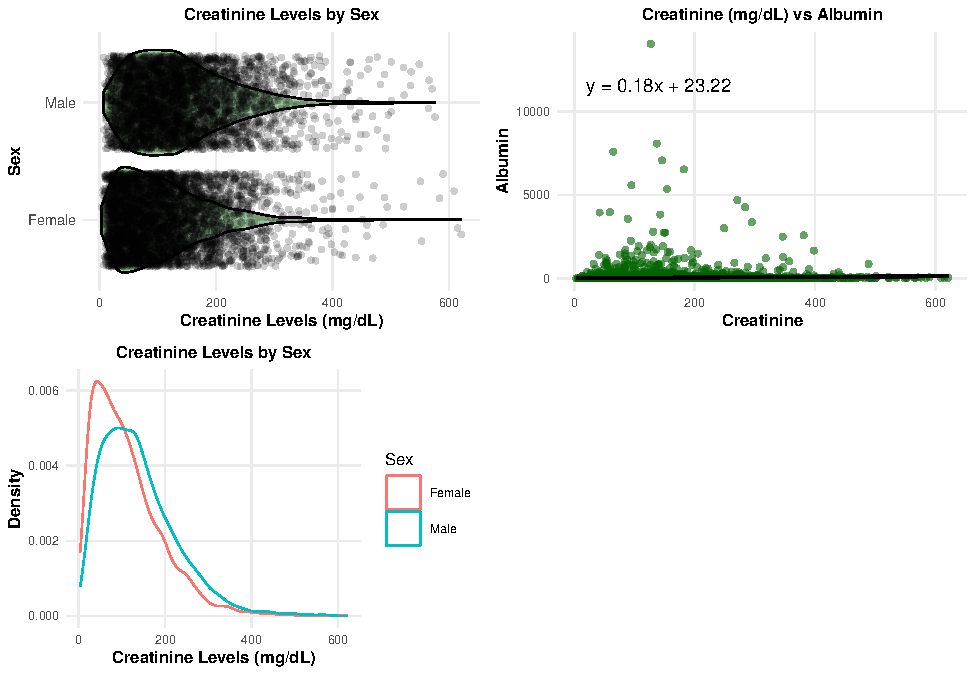
\includegraphics[keepaspectratio]{WeidnerSamuel-Assignment3_files/figure-latex/unnamed-chunk-1-1.pdf}}

\subsection{Question 3}\label{question-3}

Create a function that takes the data frame above we have been working
with, continuous variable, categorical variable, name of continuous
variable as you would like it to appear in labels and titles, and name
of categorical variable as you would like it to appear in labels and
titles. The function should create a box plot of the continuous variable
by the categorical variable. The plot should also display the p-value
comparing the results of a Wilcoxon Rank Sum Test between the
categorical variable levels. Calculate the mean and standard deviation
of the continuous variable. Using the \texttt{geom\_text()} function,
add the mean and standard deviation to the plot below the p-value. Make
sure to provide a title, appropriate labels, and colors!

\begin{Shaded}
\begin{Highlighting}[]
\CommentTok{\# Plan:}
\CommentTok{\# 1. Create a function that accepts a data frame, a continuous}
\CommentTok{\#    variable, a categorical variable, and labels for both variables}
\CommentTok{\# 2. Perform a Wilcoxon Rank Sum Test comparing the levels}
\CommentTok{\#    of the categorical variable}
\CommentTok{\# 3. Calculate the mean and standard deviation of the continuous}
\CommentTok{\#    variable within each category}
\CommentTok{\# 4. Create a box plot of the continuous variable by the}
\CommentTok{\#    categorical variable}
\CommentTok{\# 5. Add Wilcoxon p{-}value to the plot}
\CommentTok{\# 6. Add mean and standard deviation below the p{-}value.}


\NormalTok{box\_plot\_function }\OtherTok{\textless{}{-}} \ControlFlowTok{function}\NormalTok{(data, continuous\_var, categorical\_var, continuous\_name, categorical\_name) \{ }\CommentTok{\# set inputs as requested}
  
  \CommentTok{\# Remove NA data}
\NormalTok{  plot\_data }\OtherTok{\textless{}{-}}\NormalTok{ data }\SpecialCharTok{\%\textgreater{}\%}
    \FunctionTok{filter}\NormalTok{(}
      \SpecialCharTok{!}\FunctionTok{is.na}\NormalTok{(.data[[continuous\_var]]),}
      \SpecialCharTok{!}\FunctionTok{is.na}\NormalTok{(.data[[categorical\_var]])}
\NormalTok{    )}
  
  \CommentTok{\# Perform wilcoxon rank sum test}
\NormalTok{  wilcox\_result }\OtherTok{\textless{}{-}} \FunctionTok{wilcox.test}\NormalTok{(}
\NormalTok{    plot\_data[[continuous\_var]] }\SpecialCharTok{\textasciitilde{}}\NormalTok{ plot\_data[[categorical\_var]]}
\NormalTok{  )}
  
  \CommentTok{\# get p value from wilcox results}
\NormalTok{  p\_value }\OtherTok{\textless{}{-}}\NormalTok{ wilcox\_result}\SpecialCharTok{$}\NormalTok{p.value}
  
  \CommentTok{\# p value text to add to figure}
\NormalTok{  p\_label }\OtherTok{\textless{}{-}} \FunctionTok{paste0}\NormalTok{(}\StringTok{"Wilcoxon p = "}\NormalTok{, }\FunctionTok{format.pval}\NormalTok{(p\_value, }\AttributeTok{digits =} \DecValTok{3}\NormalTok{))}
  
  \CommentTok{\# calculate mean and standard deviation }
\NormalTok{  summary\_data }\OtherTok{\textless{}{-}}\NormalTok{ plot\_data }\SpecialCharTok{\%\textgreater{}\%}
    \FunctionTok{group\_by}\NormalTok{(.data[[categorical\_var]]) }\SpecialCharTok{\%\textgreater{}\%}
    \FunctionTok{summarise}\NormalTok{(}
      \AttributeTok{Mean =} \FunctionTok{mean}\NormalTok{(.data[[continuous\_var]], }\AttributeTok{na.rm =} \ConstantTok{TRUE}\NormalTok{),}
      \AttributeTok{Std\_Dev =} \FunctionTok{sd}\NormalTok{(.data[[continuous\_var]], }\AttributeTok{na.rm =} \ConstantTok{TRUE}\NormalTok{),}
      \AttributeTok{.groups =} \StringTok{"drop"}
\NormalTok{    )}
  
  \CommentTok{\# create text label for mean and standard deviation}
\NormalTok{  summary\_label }\OtherTok{\textless{}{-}} \FunctionTok{paste0}\NormalTok{(summary\_data[[categorical\_var]],}\StringTok{": Mean = "}\NormalTok{, }\FunctionTok{round}\NormalTok{(summary\_data}\SpecialCharTok{$}\NormalTok{Mean, }\DecValTok{2}\NormalTok{), }\StringTok{", Std Dev = "}\NormalTok{, }\FunctionTok{round}\NormalTok{(summary\_data}\SpecialCharTok{$}\NormalTok{Std\_Dev, }\DecValTok{2}\NormalTok{), }\AttributeTok{collapse =} \StringTok{"}\SpecialCharTok{\textbackslash{}n}\StringTok{"}\NormalTok{)}
  
  \CommentTok{\# find the max value of the continuous variable for formatting}
\NormalTok{  max\_value }\OtherTok{\textless{}{-}} \FunctionTok{max}\NormalTok{(}
\NormalTok{    plot\_data[[continuous\_var]],}
    \AttributeTok{na.rm =} \ConstantTok{TRUE}
\NormalTok{  )}
  
  \CommentTok{\# put p value above plots max value so it doesn\textquotesingle{}t block the plot}
\NormalTok{  p\_y }\OtherTok{\textless{}{-}}\NormalTok{ max\_value}\SpecialCharTok{*}\FloatTok{1.2}
  
  \CommentTok{\# put mean below the p value {-} same as above}
\NormalTok{  stats\_y}\OtherTok{\textless{}{-}}\NormalTok{ max\_value}\SpecialCharTok{*}\FloatTok{1.1}
  
  \CommentTok{\# Build box plot}
  
\NormalTok{  box\_plot }\OtherTok{\textless{}{-}} \FunctionTok{ggplot}\NormalTok{(}
\NormalTok{    plot\_data,}
    \FunctionTok{aes}\NormalTok{( }\CommentTok{\# set variables}
      \AttributeTok{x =}\NormalTok{ .data[[categorical\_var]],}
      \AttributeTok{y =}\NormalTok{ .data[[continuous\_var]],}
      \AttributeTok{fill =}\NormalTok{ .data[[categorical\_var]]}
\NormalTok{    )}
\NormalTok{  ) }\SpecialCharTok{+}
  \FunctionTok{geom\_boxplot}\NormalTok{(}
      \AttributeTok{alpha =} \FloatTok{0.7}\NormalTok{,}
      \AttributeTok{color =} \StringTok{"black"}
\NormalTok{    ) }\SpecialCharTok{+}
    \CommentTok{\# Add p{-}value}
    \FunctionTok{geom\_text}\NormalTok{( }\CommentTok{\# add text for p value}
      \FunctionTok{aes}\NormalTok{(}
        \AttributeTok{x =} \FloatTok{1.5}\NormalTok{,}
        \AttributeTok{y =}\NormalTok{ p\_y,}
        \AttributeTok{label =}\NormalTok{ p\_label}
\NormalTok{      ),}
      \AttributeTok{color =} \StringTok{"red"}\NormalTok{,}
      \AttributeTok{fontface =} \StringTok{"bold"}
\NormalTok{    ) }\SpecialCharTok{+}
    \CommentTok{\# Add mean and standard dev}
    \FunctionTok{geom\_text}\NormalTok{( }\CommentTok{\# add text for summ stats}
      \FunctionTok{aes}\NormalTok{(}
        \AttributeTok{x =} \FloatTok{1.5}\NormalTok{,}
        \AttributeTok{y =}\NormalTok{ stats\_y,}
        \AttributeTok{label =}\NormalTok{ summary\_label}
\NormalTok{      ),}
      \AttributeTok{size =} \FloatTok{3.5}
\NormalTok{    ) }\SpecialCharTok{+}
    \CommentTok{\# Add title and axis labels}
    \FunctionTok{labs}\NormalTok{(}
      \AttributeTok{title =} \FunctionTok{paste}\NormalTok{(}
\NormalTok{        continuous\_name,}
        \StringTok{"by"}\NormalTok{,}
\NormalTok{        categorical\_name}
\NormalTok{      ),}
      \AttributeTok{x =}\NormalTok{ categorical\_name,}
      \AttributeTok{y =}\NormalTok{ continuous\_name,}
      \AttributeTok{fill =}\NormalTok{ categorical\_name}
\NormalTok{    ) }\SpecialCharTok{+}
    \FunctionTok{theme\_minimal}\NormalTok{(}\AttributeTok{base\_size =} \DecValTok{8}\NormalTok{) }\SpecialCharTok{+} \CommentTok{\# set minimal theme and default size}
    \FunctionTok{theme}\NormalTok{( }\CommentTok{\# set title formatting}
      \AttributeTok{plot.title =} \FunctionTok{element\_text}\NormalTok{(}
        \AttributeTok{hjust =} \FloatTok{0.5}\NormalTok{,}
        \AttributeTok{face =} \StringTok{"bold"}\NormalTok{,}
        \AttributeTok{size =} \DecValTok{10}
\NormalTok{      ),}
      \AttributeTok{axis.title =} \FunctionTok{element\_text}\NormalTok{(}
        \AttributeTok{face =} \StringTok{"bold"} \CommentTok{\# set axis as bold}
\NormalTok{      ),}
      \AttributeTok{panel.grid.minor =} \FunctionTok{element\_blank}\NormalTok{() }\CommentTok{\# remove gridlines}
\NormalTok{    )}
  
  \CommentTok{\# Return plot}
  \FunctionTok{return}\NormalTok{(box\_plot)}
\NormalTok{\}}

\CommentTok{\# generate boxplot using functioj}
\NormalTok{box\_plot }\OtherTok{\textless{}{-}} \FunctionTok{box\_plot\_function}\NormalTok{(merged\_data, }\StringTok{"Creatinine"}\NormalTok{, }\StringTok{"Sex"}\NormalTok{, }\StringTok{"Creatinine Level"}\NormalTok{, }\StringTok{"Sex"}\NormalTok{)}

\NormalTok{box\_plot }
\end{Highlighting}
\end{Shaded}

\pandocbounded{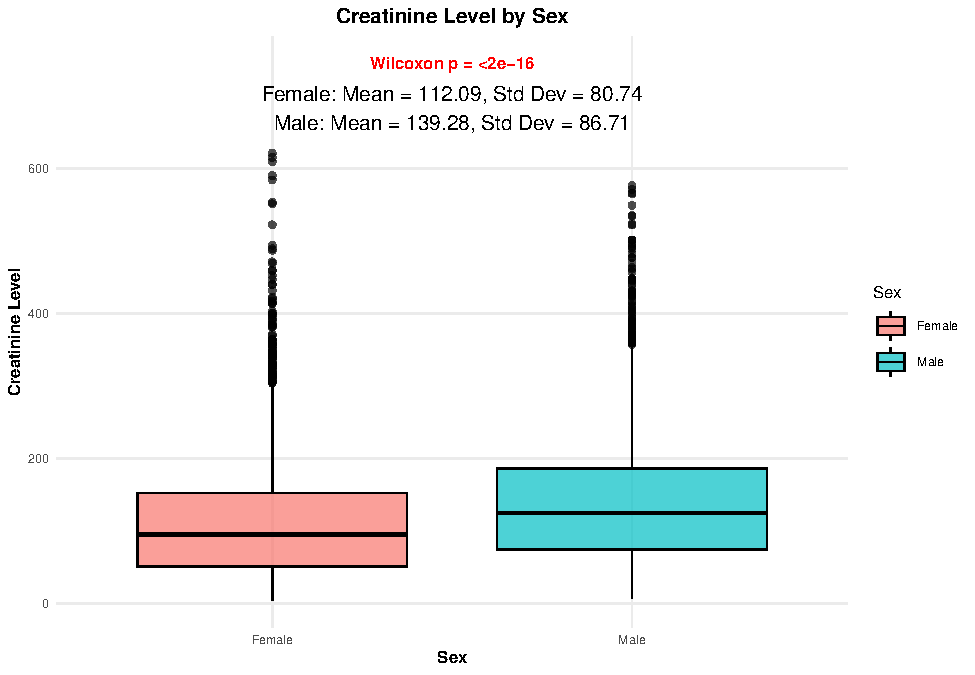
\includegraphics[keepaspectratio]{WeidnerSamuel-Assignment3_files/figure-latex/unnamed-chunk-2-1.pdf}}

\subsection{Question 4}\label{question-4}

Using a for loop, create 5 random data frames containing the following
columns:

\begin{itemize}
\tightlist
\item
  Participant ID: There should be 100 participants in each data frame
  with unique identifiers.
\item
  Sex: Sex should be comprised of two levels - Male and Female
\item
  Age: This data frame should contain only adults between 18 and 85.
\item
  Red Blood Cell Count: Female: 3.92 - 5.13 cells/L (trillion), Male:
  4.35-5.65 cells/L (trillion)
\item
  White Blood Cell Count: 3.4-9.6 cell/L (billion)
\end{itemize}

Put these data frames into a list.

\begin{Shaded}
\begin{Highlighting}[]
\CommentTok{\# Plan}
\CommentTok{\# 1. Set number of observations and initialize blank list}
\CommentTok{\# 2. Loop through a for loop five times, building a data frame each time}
\CommentTok{\#.   generating random data across the dataframe as requested. }
\CommentTok{\# 3. Add each random data frame to the blank list in each itearation of the loop}

\NormalTok{n }\OtherTok{\textless{}{-}} \DecValTok{100} \CommentTok{\# set number of observations to build out}

\CommentTok{\# Create an empty list to store the 5 data frames}
\NormalTok{blood\_cell\_data }\OtherTok{\textless{}{-}} \FunctionTok{list}\NormalTok{()}

\CommentTok{\# Loop 5 times}
\ControlFlowTok{for}\NormalTok{ (i }\ControlFlowTok{in} \DecValTok{1}\SpecialCharTok{:}\DecValTok{5}\NormalTok{) \{ }\CommentTok{\# loop over the data generation 5 times }
\NormalTok{  random\_data }\OtherTok{\textless{}{-}} \FunctionTok{data.frame}\NormalTok{(}
    \AttributeTok{Participant\_ID =} \FunctionTok{paste}\NormalTok{(}\StringTok{"pt"}\NormalTok{, }\DecValTok{1}\SpecialCharTok{:}\NormalTok{n, }\AttributeTok{sep =} \StringTok{"\_"}\NormalTok{),  }\CommentTok{\# Generate participant ids}
    \AttributeTok{Sex =} \FunctionTok{sample}\NormalTok{(}\FunctionTok{c}\NormalTok{(}\StringTok{"Male"}\NormalTok{, }\StringTok{"Female"}\NormalTok{), n, }\AttributeTok{replace =} \ConstantTok{TRUE}\NormalTok{),  }\CommentTok{\# Random sex values}
    \AttributeTok{Age =} \FunctionTok{pmax}\NormalTok{(}\DecValTok{18}\NormalTok{, }\FunctionTok{pmin}\NormalTok{(}\DecValTok{85}\NormalTok{, }\FunctionTok{round}\NormalTok{(}\FunctionTok{rnorm}\NormalTok{(n, }\AttributeTok{mean =} \DecValTok{50}\NormalTok{, }\AttributeTok{sd =} \DecValTok{10}\NormalTok{)))),  }\CommentTok{\# Random ages between 18 and 85}
    \AttributeTok{white\_blood\_cell =} \FunctionTok{runif}\NormalTok{(n, }\AttributeTok{min =} \FloatTok{3.4}\NormalTok{, }\AttributeTok{max =} \FloatTok{9.6}\NormalTok{)  }\CommentTok{\# Random WBC on uniform dist over range}
\NormalTok{  ) }\SpecialCharTok{\%\textgreater{}\%} 
  \FunctionTok{group\_by}\NormalTok{(Sex) }\SpecialCharTok{\%\textgreater{}\%} \CommentTok{\# Group by the sex variable}
  \CommentTok{\# create uniform dist over range for RBC based on sex}
  \FunctionTok{mutate}\NormalTok{(}
    \AttributeTok{red\_blood\_cell =} \ControlFlowTok{if}\NormalTok{ (}\FunctionTok{cur\_group}\NormalTok{()}\SpecialCharTok{$}\NormalTok{Sex }\SpecialCharTok{==} \StringTok{"Male"}\NormalTok{) \{}
      \FunctionTok{runif}\NormalTok{(}\FunctionTok{n}\NormalTok{(), }\AttributeTok{min =} \FloatTok{4.35}\NormalTok{, }\AttributeTok{max =} \FloatTok{5.65}\NormalTok{)}
\NormalTok{    \} }\ControlFlowTok{else}\NormalTok{ \{}
      \FunctionTok{runif}\NormalTok{(}\FunctionTok{n}\NormalTok{(), }\AttributeTok{min =} \FloatTok{3.92}\NormalTok{, }\AttributeTok{max =} \FloatTok{5.13}\NormalTok{)}
\NormalTok{    \}}
\NormalTok{  )}
\NormalTok{  blood\_cell\_data[[i]] }\OtherTok{\textless{}{-}}\NormalTok{ random\_data }\CommentTok{\# use the index variable to add dataframe to my list}
\NormalTok{\}}
\end{Highlighting}
\end{Shaded}

\subsection{Question 5}\label{question-5}

For each of the data frames you generated in the previous question,
create a scatter plot with the red blood cell count on the x-axis and
the white blood cell count on the y-axis. Color the points by Sex. Once
you have created these plots, arrange the plots in a panel using
\texttt{ggarrange()}. Hint: Make a list of the plots that you can apply
to the function \texttt{do.call()} along with \texttt{ggarrange()}!

\begin{Shaded}
\begin{Highlighting}[]
\CommentTok{\# Plan}
\CommentTok{\# 1. Use lapply to apply my list of dataframes to a function that plots scatter plots }
\CommentTok{\# 2. Use do.call() to apply the list of the scatter plots within the ggarrange function to make a panel of plots}

\CommentTok{\# write scatter plot }
\NormalTok{scatter\_plots\_blood\_cells }\OtherTok{\textless{}{-}} \FunctionTok{lapply}\NormalTok{( }\CommentTok{\# apply list to function}
\NormalTok{  blood\_cell\_data,}
  \ControlFlowTok{function}\NormalTok{(data) \{}
    \FunctionTok{ggplot}\NormalTok{(}
\NormalTok{      data,}
      \FunctionTok{aes}\NormalTok{(}
        \AttributeTok{x =}\NormalTok{ red\_blood\_cell,}
        \AttributeTok{y =}\NormalTok{ white\_blood\_cell,}
        \AttributeTok{color =}\NormalTok{ Sex }\CommentTok{\# set grouped coloring }
\NormalTok{      )}
\NormalTok{    ) }\SpecialCharTok{+}
      \FunctionTok{geom\_point}\NormalTok{(}
        \AttributeTok{alpha =} \FloatTok{0.8} \CommentTok{\# set transparency and add points for scatter}
\NormalTok{      ) }\SpecialCharTok{+}
      \FunctionTok{labs}\NormalTok{( }\CommentTok{\# set labels for x y and title}
        \AttributeTok{title =} \StringTok{"Red Blood Cell vs White Blood Cell Count"}\NormalTok{,}
        \AttributeTok{x =} \StringTok{"RBC Count cells/L (trillion)"}\NormalTok{,}
        \AttributeTok{y =} \StringTok{"WBC Count cells/L (billion)"}\NormalTok{,}
        \AttributeTok{color =} \StringTok{"Sex"}
\NormalTok{      ) }\SpecialCharTok{+}
      \FunctionTok{theme\_minimal}\NormalTok{(}\AttributeTok{base\_size =} \DecValTok{8}\NormalTok{) }\SpecialCharTok{+} \CommentTok{\# set default size and minial theme}
      \FunctionTok{theme}\NormalTok{( }\CommentTok{\# set title formatting}
        \AttributeTok{plot.title =} \FunctionTok{element\_text}\NormalTok{(}
          \AttributeTok{hjust =} \FloatTok{0.5}\NormalTok{,}
          \AttributeTok{face =} \StringTok{"bold"}\NormalTok{,}
          \AttributeTok{size =} \DecValTok{8}
\NormalTok{        ),}
        \AttributeTok{axis.title =} \FunctionTok{element\_text}\NormalTok{( }\CommentTok{\# set axis formatting}
          \AttributeTok{face =} \StringTok{"bold"}\NormalTok{,}
          \AttributeTok{size =} \DecValTok{4}
\NormalTok{        ),}
        \AttributeTok{panel.grid.minor =} \FunctionTok{element\_blank}\NormalTok{(), }\CommentTok{\# remove grid lines}
        \AttributeTok{legend.text =} \FunctionTok{element\_text}\NormalTok{(}\AttributeTok{size =} \DecValTok{6}\NormalTok{),}
        \AttributeTok{legend.title =} \FunctionTok{element\_text}\NormalTok{(}\AttributeTok{size =} \DecValTok{8}\NormalTok{)}
\NormalTok{      )}
\NormalTok{  \}}
\NormalTok{)}

\FunctionTok{do.call}\NormalTok{( }\CommentTok{\# apply ggarrange() across the list of scatter plots}
\NormalTok{  ggarrange,}
  \FunctionTok{c}\NormalTok{(scatter\_plots\_blood\_cells, }\AttributeTok{ncol =} \DecValTok{2}\NormalTok{, }\AttributeTok{nrow =} \DecValTok{3}\NormalTok{,}\AttributeTok{spacing =} \DecValTok{1}\NormalTok{), }\CommentTok{\# add spacing for no overlap}
\NormalTok{)}
\end{Highlighting}
\end{Shaded}

\pandocbounded{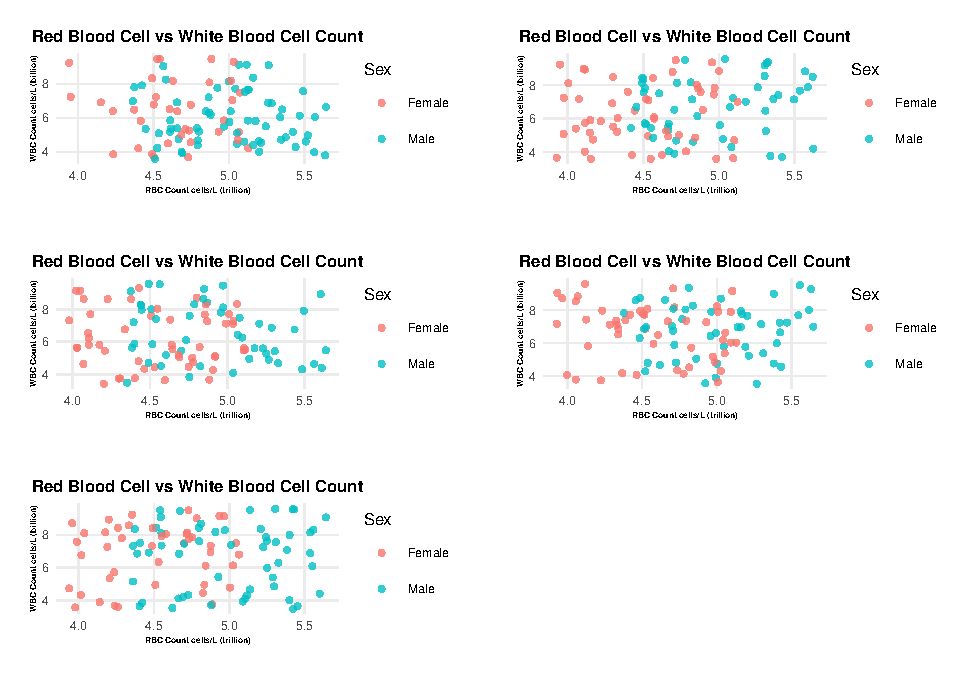
\includegraphics[keepaspectratio]{WeidnerSamuel-Assignment3_files/figure-latex/unnamed-chunk-4-1.pdf}}

\end{document}
